
\documentclass[ms.tex]{subfiles}
\begin{document}

\section{Mock Samples}
\label{sec:mocks}

\subsection{A Fiducial Mock Sample}
\label{sec:mocks:fiducial}

\begin{figure*}
\centering
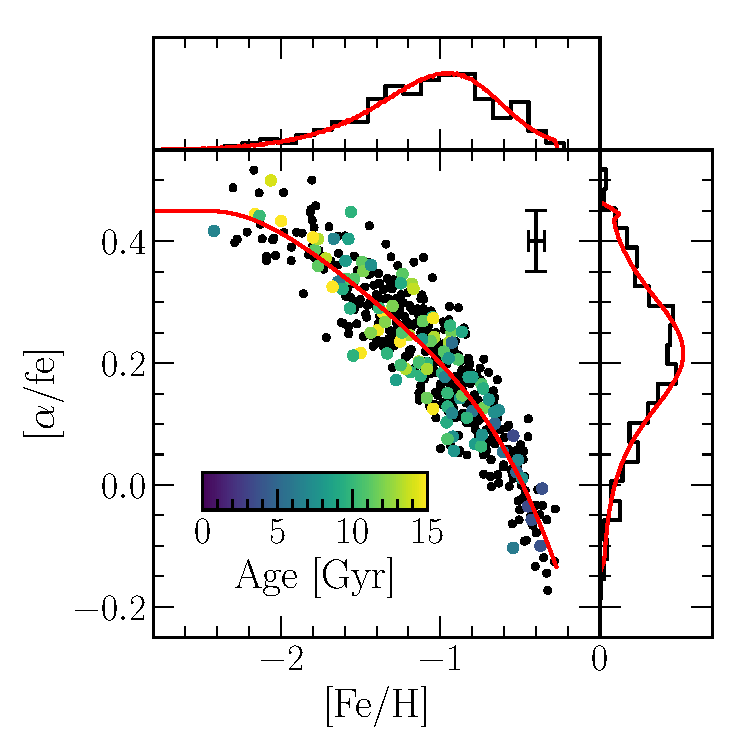
\includegraphics[scale = 0.5]{fiducial_mock_afe_feh.pdf}
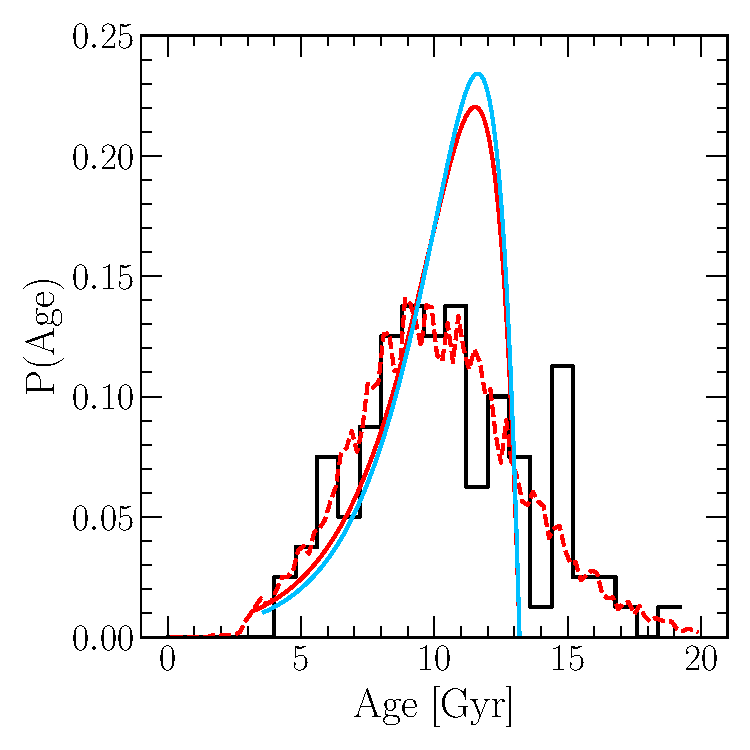
\includegraphics[scale = 0.42]{fiducial_mock_agedist.pdf}
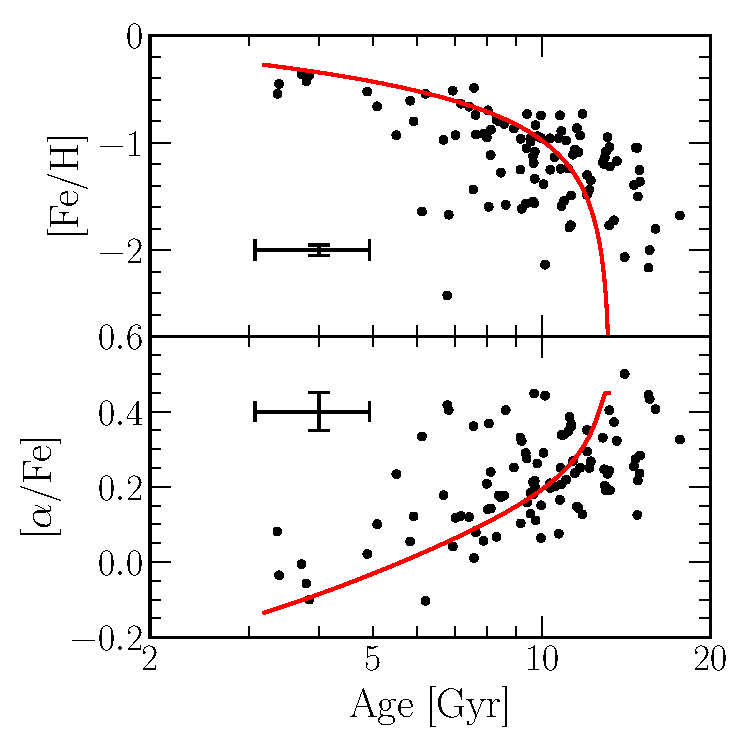
\includegraphics[scale = 0.42]{fiducial_mock_amr.pdf}
\caption{
\textbf{Left}: Our fiducial mock sample in the~\afe-\feh~plane.
There are~$N = 500$ stars with abundance uncertainties
of~$\sigma(\feh) = \sigma(\afe) = 0.05$ as indicated by the errorbar.
$N = 100$ of the stars have age information available with an artificial
uncertainty of~$\sigma(\log_{10}(\text{age})) = 0.1$ as indicated by the
colorbar.
The red line denotes the evolutionary track in the gas-phase from the one-zone
model that generated the mock.
On the top and right, we show the marginalized distributions
in~\afe~and~\feh, with red lines denoting the known distribution.
\textbf{Center}: The mock (black, binned) and known (red) age distributions.
The dashed red line indicates the age distribution that is obtained by sampling
$N = 10^4$ rather than $N = 500$ stars and assuming the same age uncertainty
of~$\sigma(\log_{10}(\text{age})) = 0.1$.
\textbf{Right}: The age-\feh~(top) and age-\afe~(bottom) relation for the mock
sample, with artificial uncertainties denoted by the error bars on each panel.
The red lines denotes the known relations for the gas-phase.
}
\label{fig:fiducialmock}
\end{figure*}

% \begin{table}
% \caption{
% The known parameters of the one-zone model from which we generate our mock
% stellar samples.
% }
% \begin{tabularx}{\columnwidth}{l @{\extracolsep{\fill}} l r}
% \hline
% Parameter & Description & Value
% \\
% \hline
% $\tau_\text{in}$ & e-folding timescale of the infall history & 2 Gyr
% \\
% $\eta$ & Outflow mass-loading factor
% ($\eta \equiv \dot{M}_\text{out} / \dot{M}_\star$) & 10
% \\
% $\tau_\star$ & SFE timescale ($\tau_\star \equiv M_\text{g} / \dot{M}_\star$) &
% 15 Gyr
% \\
% $\tau_\text{tot}$ & Duration of star formation & 10 Gyr
% \\
% \yfecc & IMF-averaged fractional net Fe yield from CCSNe & 0.0008
% \\
% \yfeia & IMF-averaged fractional net Fe yield from SN Ia & 0.0011
% \\
% \hline
% \end{tabularx}
% \label{tab:fiducial_mock_params}
% \end{table}

\begin{itemize}

	\item We use our parametrization of one-zone GCE models described
	in~\S~\ref{sec:methods:onezone} to set up an underlying model from which
	mock samples can be drawn; we then use a fiducial mock sample to describe
	our fitting method in~\S~\ref{sec:methods:fitting} and explore variations
	in, e.g., sample size and precision.

	\item We take an exponential infall history described by
	\begin{equation}
	\dot{M}_\text{in} \propto e^{-t/\tau_\text{in}}
	\end{equation}
	with~$\tau_\text{in} = 2$ Gyr and an initial gas mass of 0.
	The overall normalization of the infall history is irrelevant because
	mass information cancels in one-zone models when you compute abundances.
	We additionally select~$\tau_\star = 15$ Gyr and~$\eta = 10$ with the
	thought that slow star formation and strong outflows would mimic the
	evolution seen in a typical field dwarf galaxy.
	We set the onset of star formation~$\tau = 13.2$ Gyr ago, allowing~$\sim$0.5
	Gyr between the Big Bang and the first stars.
	We evolve this model for 10 Gyr (i.e. the exact ages of the youngest stars
	in the mock sample are~$\tau = 3.2$ Gyr).

	\item {\color{red} YIELDS}

	\item One-zone models produce stellar populations rather than individual
	stars, so if a mock sample of individual stars is to be obtained, we must
	sample from the underlying population.
	Higher mass stellar populations have proportionally more stars than lower
	mass stellar populations, so we take the probability of sampling to be
	proportional to the mass of a population.
	In the interest of mimicing typical observational samples for local group
	dwarfs, we take~$N = 500$ stars with abundance uncertainties of
	$\sigma\afe = \sigma\feh = 0.05$.
	100 of these stars have age information with an uncertainty
	of~$\sigma\logage = 0.1$.

	\item We illustrate this sample in Fig.~\ref{fig:fiducialmock}.
	This sample shows a ``knee'' in the~\afe-\feh~diagram near~\feh~$\sim$-2.3
	and an equilibrium abundance near~\feh~$\sim$-0.3, but due to the
	declining nature of the SFH, most of the stars form in
	the~\feh~$\sim$-1 and~\afe~$\sim$+0.2 region of chemical space.

\end{itemize}

\subsection{Recovered Parameters of the Fiducial Mock}
\label{sec:mocks:fiducial_fit}

\begin{figure*}
\centering
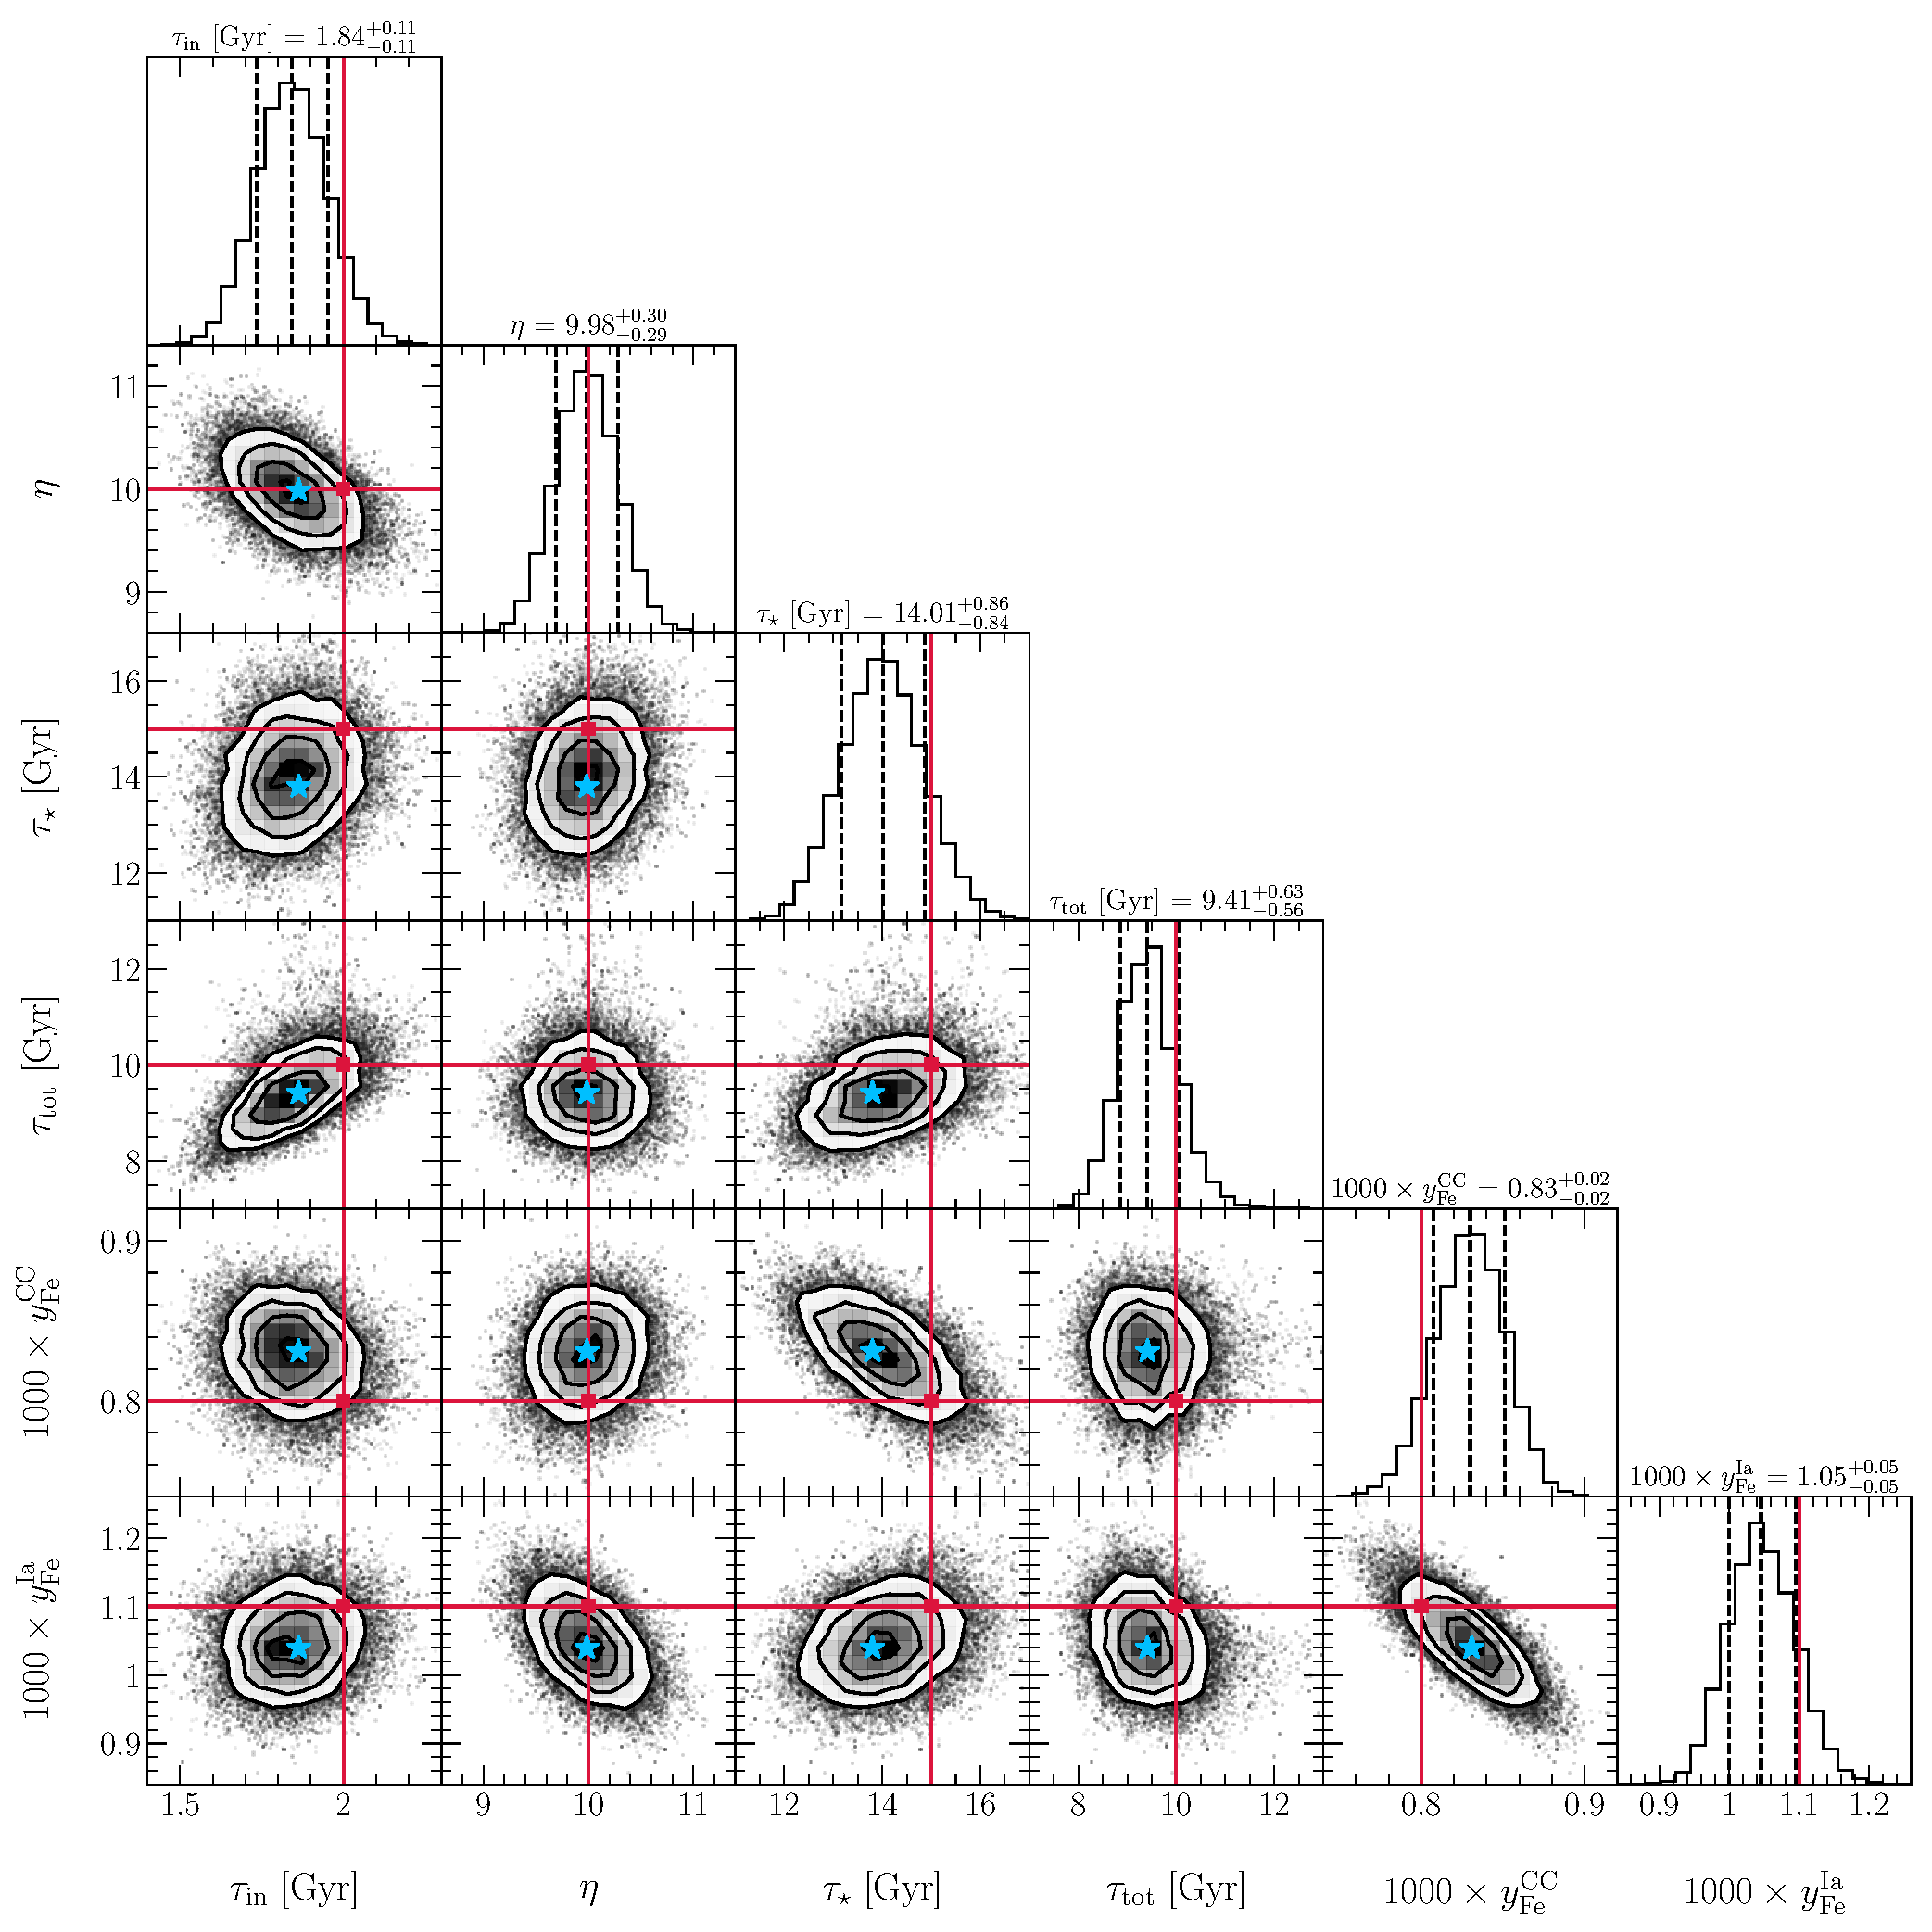
\includegraphics[scale = 0.45]{fiducial_76k8.pdf}
\caption{
The ``corner-plot'' showing the results of applying our fitting method to our
fiducial mock sample (see discussion in~\S\S~\ref{sec:methods:fitting}
and~\ref{sec:mocks:fiducial}).
We show the marginalized likelihood distributions in each parameter along with
their best-fit values and confidence intervals along the diagonal.
Below the diagonal, we show the 2-dimensional cross-sections of the
6-dimensional likelihood function.
Blue stars mark the element of the Markov Chain with the maximum likelihood.
Red ``cross-hairs'' denote the true, known values of the parameters which were
used to generate the mock sample (see the top row of
Table~\ref{tab:recovered_values}).
}
\label{fig:corner_fiducial}
\end{figure*}

\begin{itemize}

	\item We apply the method outlined in~\S~\ref{sec:methods:fitting} to the
	mock sample detailed in~\S~\ref{sec:mocks:fiducial}.
	Fig.~\ref{fig:corner_fiducial} shows the ``corner-plot'' derived from this
	procedure.
	Along the diagonal, we show the marginalized likelihood distributions in
	each parameter along with their best-fit values and confidence intervals.
	Below the diagonal, we show 2-dimensional cross-sections of the
	6-dimensional likelihood function.
	Blue stars mark the element of the Markov Chain with the highest value
	of~$\ln L$, and red ``cross-hairs'' denote the true, known values of the
	parameters from the mock sample (see the top row of
	Table~\ref{tab:recovered_values}).

	\item Our fitting method is able to accurately recover the known
	evolutionary parameters of the mock sample.
	Although it may appear that there are a high number of~$\gtrsim1\sigma$
	discrepancies, we demonstrate in~\S~

	\item We note a handful of degeneracies in the likelihood distributions of
	the recovered parameters.
	{\color{red}
	Because some of these degeneracies arise from similar physics, this
	discussion can be shortened significantly by motivating items from that
	perspective rather than going through panel-by-panel.
	}

	\begin{itemize}

		\item[\textbf{1.}] There is an inverse relationship between the
		derived Fe yields from CCSN and SN Ia.
		This is expected, because for the fixed~$\alpha$ yield of~\yacc~= 0.01,
		the total yield of Fe is constrained by the~\feh~MDF, and for a high
		(low) value of~\yfecc, a low (high) value of~\yfeia~is required to
		make up the difference between the model and the data.

		\item[\textbf{2.}] There is an inverse relationship between the prompt
		component of the Fe yield~\yfecc~and the SFE timescale~$\tau_\star$.
		This arises because~$\tau_\star$ is the parameter which plays the
		dominant role in establishing the position of the ``knee'' in
		the~\afe-\feh~diagram by influencing the rate of enrichment at early
		times~\citep[see discussion in][]{Weinberg2017}.
		For high (low) values of~\yfecc, a low (high) value of~$\tau_\star$ is
		required in order to place the knee at a position consistent with the
		data.

		\item[\textbf{3.}] There is a direct relationship between the infall
		timescale~$\tau_\text{in}$ and the total duration of star formation
		$\tau_\text{tot}$.
		This arises because both affect the high-metallicity tail of the~\feh
		distribution similarly.
		With shorter~$\tau_\text{in}$, the gas supply and the SFH drop off more
		sharply.
		This increases the~\feh~equilibrium abundance by allowing SNe Ia to
		enrich a ``gas-starved'' ISM~\citep[see discussion in][]{Weinberg2017},
		thereby increasing the fraction of high~\feh~stars.
		To make up this potential difference with the data, the model can shut
		off star formation earlier, cutting off the high-metallicity end of
		the~\feh~MDF, giving rise to this direct relationship.

		\item[\textbf{4.}] There is an inverse relationship between the infall
		timescale and the mass loading factor~$\eta$.
		This arises because both affect the equilibrium abundance in the same
		manner.
		As discussed above, shorter values of~$\tau_\text{in}$ increase the
		equilibrium Fe abundance slightly by allowing SNe Ia to enrich a
		``gas-starved'' ISM.
		To make up for this potential discrepancy with the data, one can
		strengthen outflows by increasing~$\eta$, decreasing the equilibrium
		abundance.

		\item[\textbf{5.}] There is a degeneracy between the total duration of
		star formation~$\tau_\text{tot}$ and the SFE timescale~$\tau_\star$.
		This arises because both affect the shape of the~\feh~MDF.
		Fe approaches equilibrium on either the SFE timescale~$\tau_\star$ or
		the SN Ia DTD characteristic timescale - whichever is longer, which for
		dwarf galaxies with inefficient star formation, is~$\tau_\star$.
		As a result, higher~$\tau_\star$ models approach equilibrium faster.
		To avoid overpredicting the frequency of near-equilibrium stars
		compared to the data, one can simply cut off star formation earlier,
		thereby increasing the frequency of lower metallicity stars.

		\item[\textbf{6.}] There is a degeneracy between the mass-loading
		factor~$\eta$ and the SN Ia Fe yield~\yfeia.
		This arises because the two parameters both impact the location of the
		track in the~\afe-\feh~plane.
		With all other parameters held fixed, higher (lower) values of~\yfeia
		lower (raise) the track by increasing the denominator of~\afe.
		This potential discrepancy with the data can be mitigated by lowering
		(raising)~$\eta$, which moves the track to the left (right).

	\end{itemize}

	\item There are additional, weaker degeneracies which can be understood
	by confounding variables.
	For example, the degeneracy between~$\tau_\star$ and~\yfeia~arises because
	both are degenerate with~\yfecc.

	\item We remind the reader that our fits achieve such a precision by
	selecting a scale on which the~$\alpha$ element yield~\yacc~is defined to
	be exactly 0.01 (see discussion in~\S~\ref{sec:methods:onezone:yields}).
	Aside from the infall timescale~$\tau_\text{in}$ and the total duration of
	star formation~$\tau_\text{tot}$, each parameter in this fit is affected by
	the yield-outflow degeneracy.
	We quantify this in detail in Appendix X.

\end{itemize}

\subsection{Variations in Sample Size, Measurement Precision, and the
Availability of Age Information}
\label{sec:mocks:variations}

\subfile{mocksamples.tablebody.tex}

\begin{figure*}
\centering
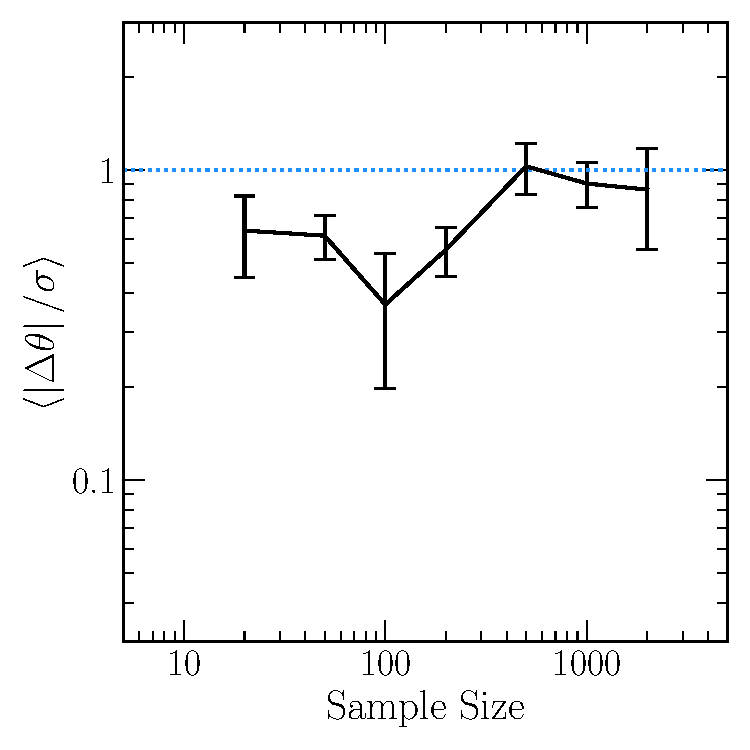
\includegraphics[scale = 0.45]{dp_sigma_samplesize.pdf}
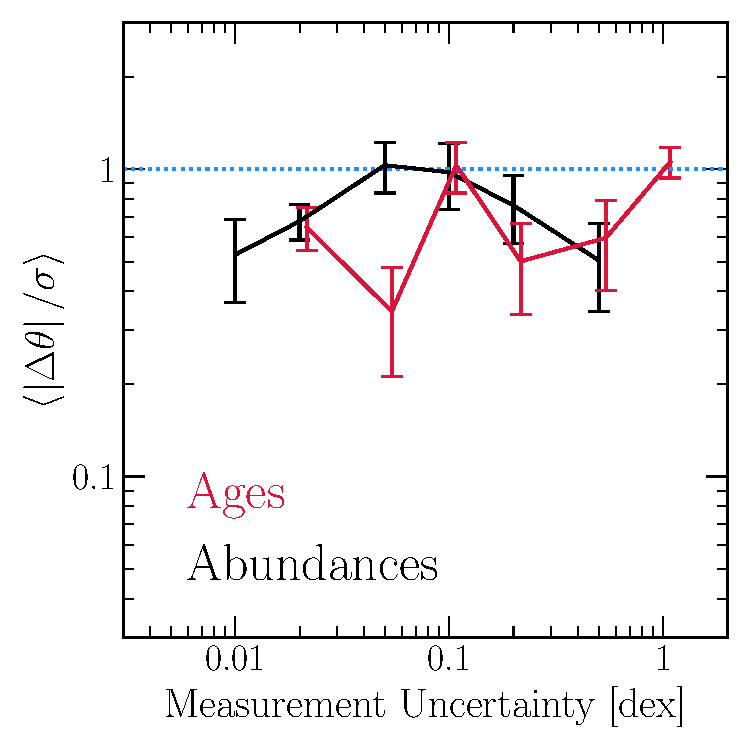
\includegraphics[scale = 0.45]{dp_sigma_precision.pdf}
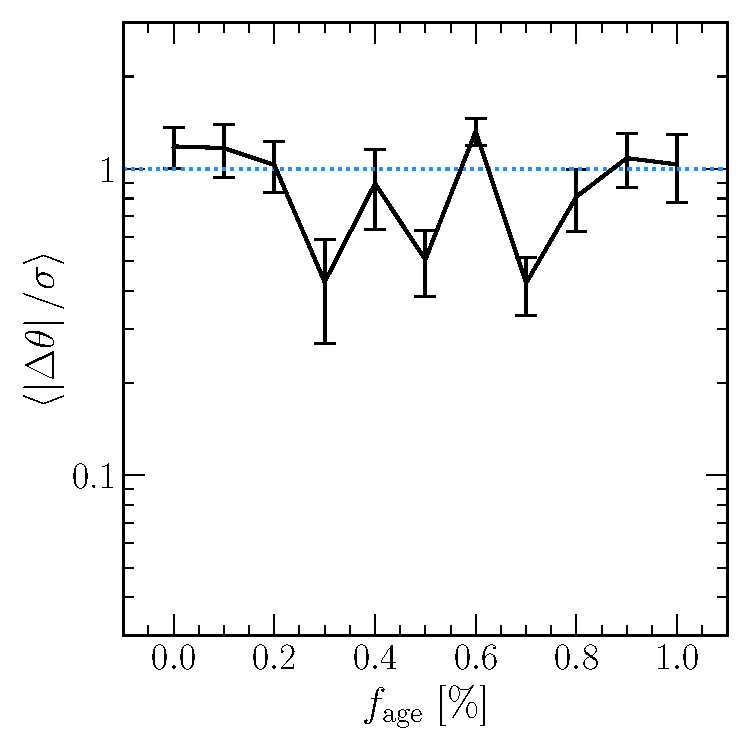
\includegraphics[scale = 0.45]{dp_sigma_agefrac.pdf}
\caption{
The mean deviation between the re-derived mock sample parameters~$\{\theta\} =
\{\tau_\text{in},~\eta,~\tau_\star,~\tau_\text{tot},~\yfecc,~\yfeia\}$ and
their known values from the mock sample in units of the uncertainty on the
best-fit values as a function of the sample size of the mock (left),
measurement precision in abundances~\feh~and~\afe (middle, black),
measurement precision in~$\log_{10}(\text{age})$ (middle, red),
and the fraction of the sample with available age information (right).
Error bars denote the error on the mean deviation in the six parameters.
Blue dotted lines mark~$\langle\Delta\theta/\sigma\rangle = 1$, the
expected value of the mean deviation for a Gaussian random process.
}
\label{fig:dp_sigma}
\end{figure*}

\begin{figure*}
\centering
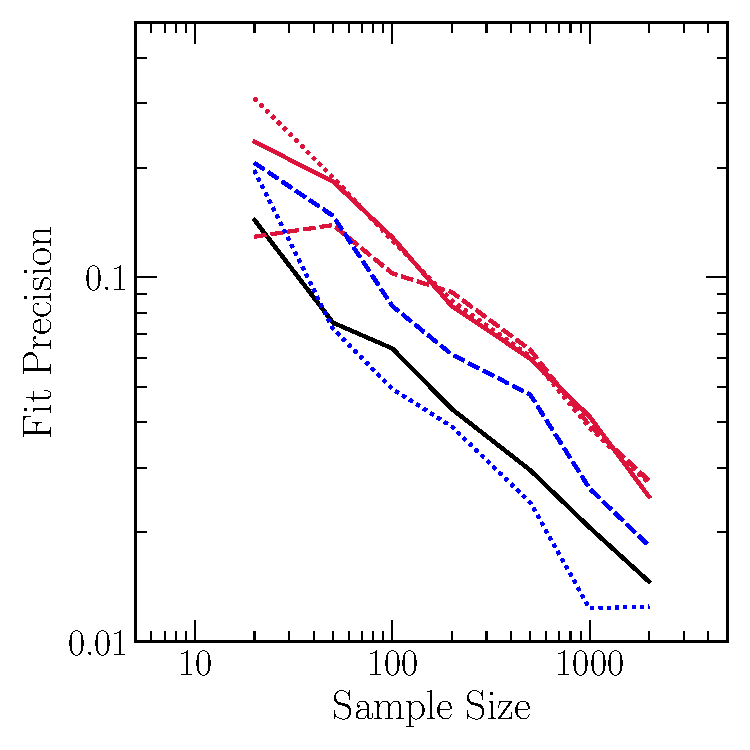
\includegraphics[scale = 0.52]{precision_samplesize.pdf}
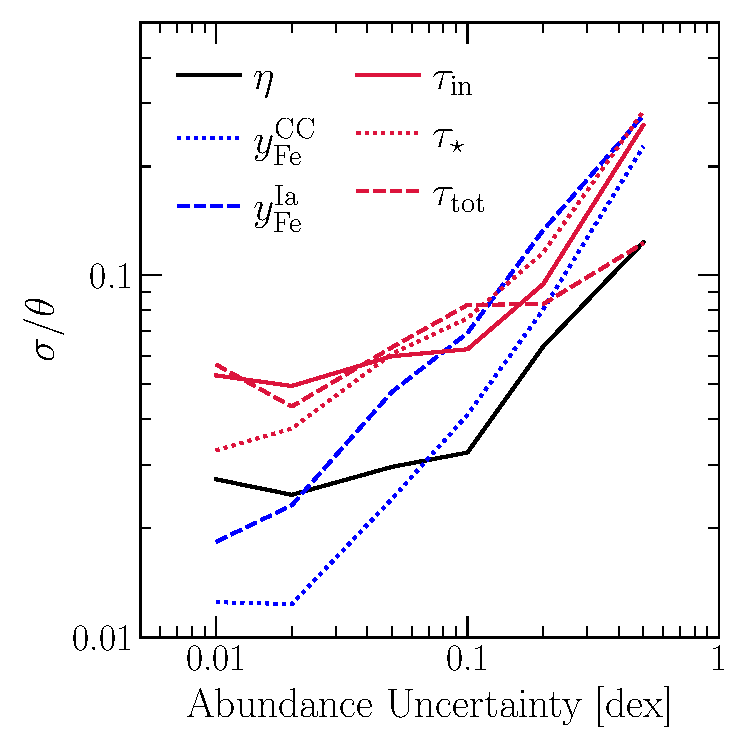
\includegraphics[scale = 0.52]{precision_abundanceuncertainty.pdf}
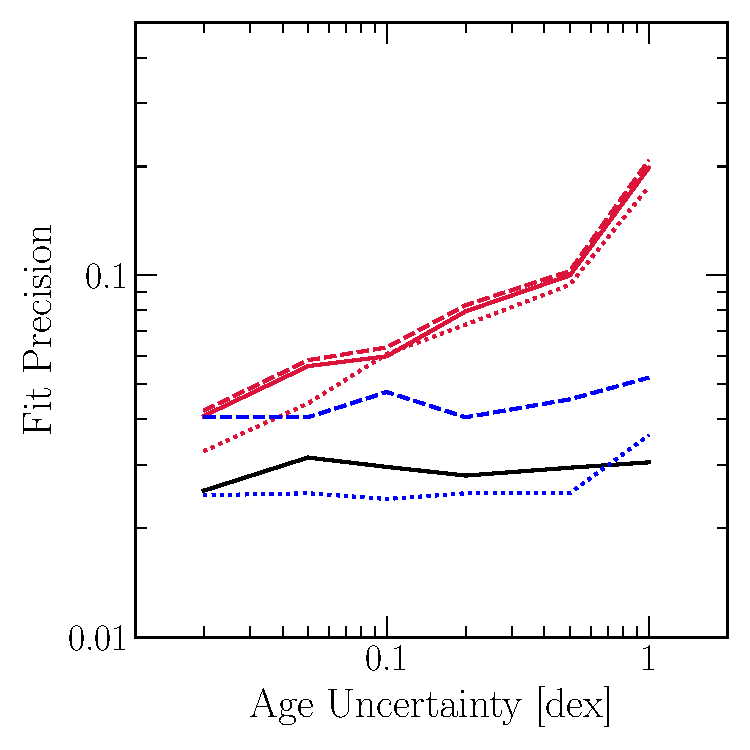
\includegraphics[scale = 0.52]{precision_ageuncertainty.pdf}
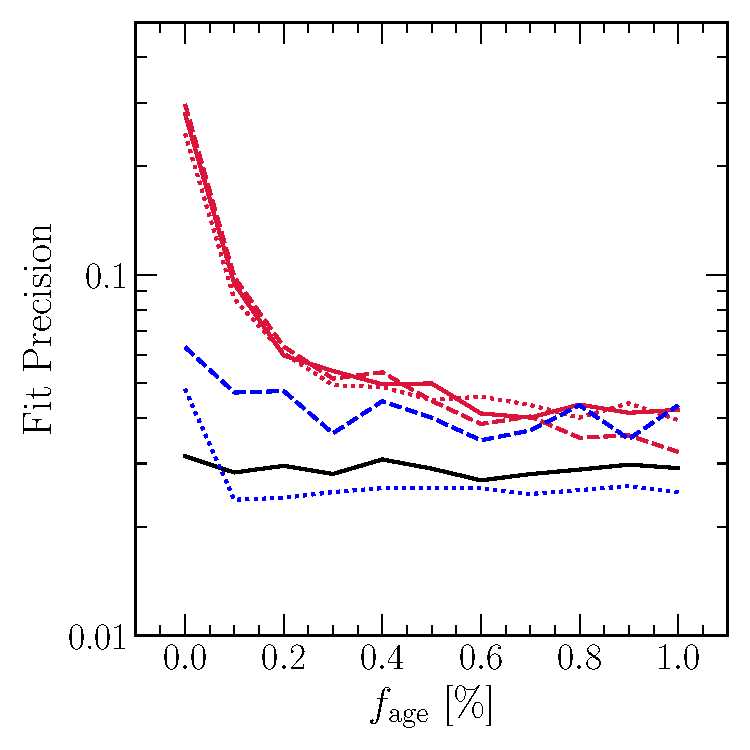
\includegraphics[scale = 0.52]{precision_agefrac.pdf}
\caption{
The precision of our re-derived mock sample parameters~$\{\theta\} =
\{\tau_\text{in},~\eta,~\tau_\star,~\tau_\text{tot},~\yfecc,~\yfeia\}$ as a
function of sample size (top left), measurement uncertainty in~\feh~and~\afe
abundances (top right), measurement uncertainty in~$\log_{10}(\text{age})$
(bottom left), and the fraction of the sample with age measurements (bottom
right).
We highlight the mass-loading factor~$\eta$ (solid black), the total duration
of the model~$\tau_\text{tot}$ (dashed green), the CCSN Fe yield~\yfecc~(dotted
red), and the SN Ia Fe yield~\yfeia~(dot-dashed blue).
The infall timescale~$\tau_\text{in}$ and the SFE timescale~$\tau_\star$ behave
similarly, so we leave them both as grey lines for visual clarity.
}
\label{fig:precision}
\end{figure*}

\begin{itemize}

	\item We now explore variations of our fiducial mock sample with respect
	to sample size, measurement precision, and the availability of age
	information.
	These variations retain all of the evolutionary parameters of the fiducial
	mock, but differ in one of the number of stars in the sample, measurement
	uncertainty in~\feh~and~\afe~abundances, measurement uncertainty
	in~$\log_{10}(\text{age})$, or the fraction of the sample with age
	measurements.
	The left-hand column of Table~\ref{tab:recovered_values} provides a summary
	of the values we take as exploratory cases for each mock variation, with
	the values taken in the fiducial sample highlighted in bold.
	In the remaining columns, we provide the associated values derived for each
	GCE parameter~$\theta$ along with their~$1\sigma$ uncertainties; the true
	values are noted in the top row.
	Our choices in measurement precision are intended to reflect typical values
	achieved by modern spectroscopic surveys where robust age information is
	often available for only a portion of the sample, and may be adopted from
	another source with a precision that is unrelated to the abundance
	uncertainties.
	Our chosen sample sizes are also intended to reflect a typical sample that
	might accurately be described by a one-zone model; with the requirement
	that mixing be efficient, it is likely that only dwarf galaxies meet this
	condition.
	Much more distant than nearby Galactic stars, dwarf galaxies are less
	conducive to the large sample sizes achieved by surveys of the Milky Way
	(e.g. APOGEE and GALAH).
	In larger systems like the Milky Way, processes such as stellar migration
	(refs) and radial gas flows (though perhaps less importantly; refs) have
	been demonstrated to significantly impact the observed abundance
	distributions as well as their evolution.
	This demands a more sophisticated parametrization than a one-zone model
	anyway, prompting a number of authors to explore so-called ``multi-zone''
	GCE models (refs).

	\item Fig.~\ref{fig:dp_sigma} demonstrates the accuracy of our fitting
	method with respect to variations in these details surrounding the data.
	On the y-axis of each panel, we plot the mean deviation between each
	re-derived parameter~$\theta$ (i.e.~$\tau_\text{in}$,~$\eta$,~$\tau_\star$,
	etc.) and its known value from the mock sample normalized according to the
	fit precision on~$\theta$.
	Under all mock variants that we explore, our method recovers the known
	values of the parameters to~$\sim1\sigma$ or slightly better.
	This is exactly as expected when the uncertainties are described by a
	Gaussian random process, for which the most likely deviation from the true
	value is exactly~$1\sigma$, even with infinite data.

	\item This suggests that our method should provide accurate best-fit
	evolutionary parameters even when the sample size is as low
	as~$N \approx 20$, when the measurement uncertainties are as high
	as~$\sigma_\text{[X/Y]} \approx 0.5$ and~$\sigma_\text{log(age)} \approx 1$,
	or even when there is no age information available at all.
	The precision of the fit will indeed suffer in these cases (see Fig.
	\ref{fig:precision} and associated discussion below), but it will remain
	accurate.

	\item We have explored alternate parametrizations of our mock sample's
	evolutionary history and indeed found that our method accurately recovers
	the parameters in each case.
	These ``stress tests'' include a case in which we build in a significant
	starburst, and our method accurately recovers both the timing and the
	strength of the burst.
	We have also explored an infall rate which varies sinusoidally about some
	mean value, mimicing a series of minor starbursts.
	Although idealized and potentially unrealistic, our method accurately
	recovers the amplitude, phase, and frequency in this case as well.
 

\end{itemize}

\end{document}



























